\chapter{Design og Implementering}

\section{Valg og Begrundelse}

\section{Hardware}

\subsection{Motorstyring}

\subsection{Affyringsmekanisme}

\section{Software}

\subsection{I2C}
I dette afsnit vil softwaren der omhandler I2C-kommunikation blive beskrevet. Dette inkluderer et klassediagram, samt en klassebeskrivelse.
\subsubsection{Klassediagram}
På figur \ref{figure:klassediagramI2CCommunication} ses klassediagrammet for I2CCommunication. 
\begin{figure}[H]
	\centering
	%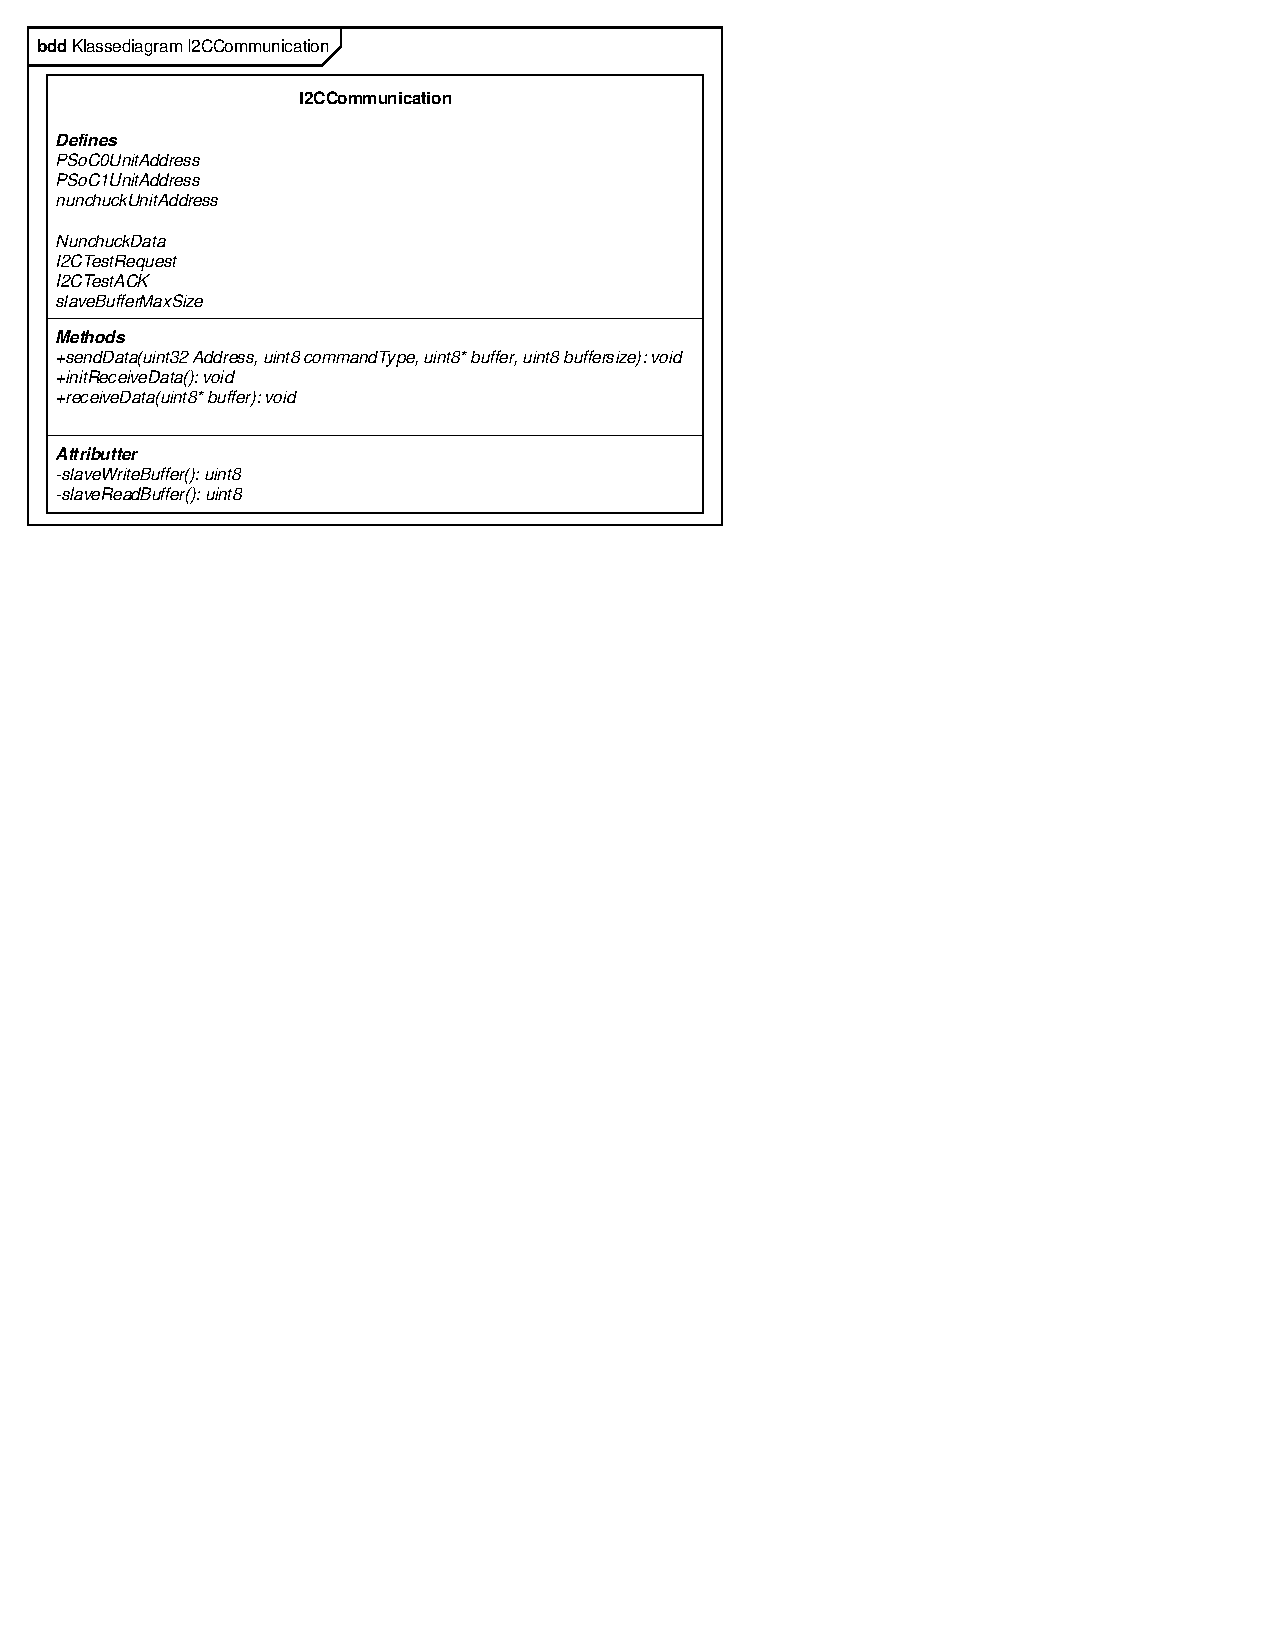
\includegraphics[width=0.9\textwidth, trim={0 19cm 9cm 0},clip]{DesignOgImplementering/images/I2CCommunication.pdf}
	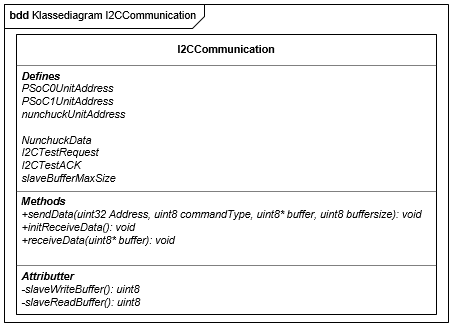
\includegraphics[]{DesignOgImplementering/images/I2CCommunication}
	%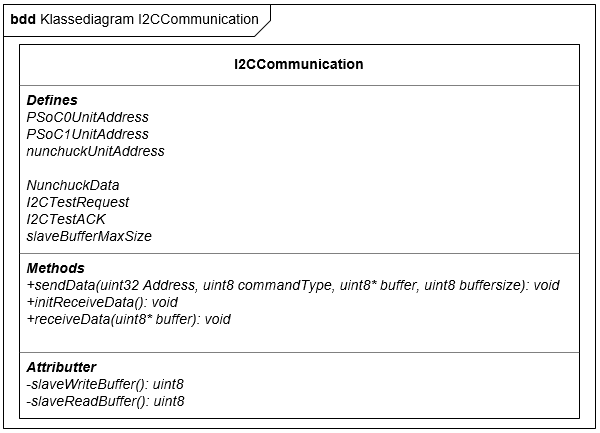
\includegraphics[width =0.9\textwidth]{DesignOgImplementering/images/I2CCommunication2}
	\caption{Klassediagram for I2CCommunication klassen}
	\label{figure:klassediagramI2CCommunication}
\end{figure}

\subsubsection{Klassebeskrivelser}
Som det ses på klassediagrammet figur \ref{figure:klassediagramI2CCommunication} indeholder klassen flere metoder. Disse metoder blive beskrevet her.\newline

\noindent\textbf{void sendData(uint8 Address, uint8 commandType, uint8* buffer, uint8 buffersize)}\newline
Denne metode sender, via PSoC Creators I2C-API, den data der ligger i "buffer" af kommandotypen "commandType" til slaven med adressen "Address". \newline

\noindent\textbf{void initReceiveData()} \newline 
Denne metode initialiserer de to buffers (slaveWrite og slaveRead) der kræves på en I2C-slave, for at kunne gøre bruge af PSoC Creator's I2C-API. \newline

\noindent\textbf{void receiveData(uint8* buffer)}\newline
Denne metode venter på at slaveRead bufferen er blevet fyldt. Når dette er sket, bliver slaveRead bufferen kopieret over i "buffer".   

\subsection{Nunchuck}
I dette afsnit vil softwaren der specifikt omhandler kommunikationen mellem PSoC0 og Nunchucken blive beskrevet. Dette gøres vha. et klassediagram og klassebeskrivelser.

\subsubsection{Klassediagram}
På figur \ref{figure:NunchuckKlassediagram} ses klassediagrammet for Nunchuck klassen.

\begin{figure}[H]
	\centering
	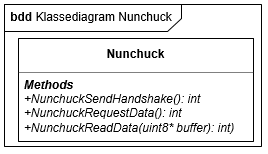
\includegraphics[]{DesignOgImplementering/images/nunchuck}
	\caption{Klassediagram for klassen Nunchuck}
	\label{figure:NunchuckKlassediagram}
\end{figure}

\subsubsection{Klassebeskrivelser}
Metoderne fra klassediagrammet figur \ref{figure:NunchuckKlassediagram} vil blive beskrevet i dette afsnit.

\noindent\textbf{int NunchuckSendHandshake()}\newline
Denne metode sender et "handshake" (Se dokumentationen afsnit \textbf{INSERT AFSNIT HER \#ref}) til Nunchuck enheden. Handshaket bruges til at "parre" PSoC'en med nunchucken. Metoden returnerer et '0' hvis der opstår en fejl. \newline

\noindent\textbf{int NunchuckRequestData()}\newline
Denne metode sender et 0x00 til nunchuck'en, og derved beder nunchuck'en om at klargøre data til overførsel. Metoden returnerer et '0' hvis der opstår en fejl. \newline

\noindent\textbf{int NunchuckreadData(uint8* buffer)}\newline
Denne metode bruger PSoC Creator's I2C-API til at læse data fra nunchuck'en (data der blev klargjort fra NunchuckRequestData()). Disse data bliver derefter dekrypteret og gemt i "buffer", så de bliver tilgængelige uden for metodens scope. \newline

I klassediagrammet er der en sektion kaldet "Defines". Disse Defines bruges i implementeringen til forskellige formål. \textit{PSoC0UnitAddress, PSoC1UnitAddres} og \textit{nunchuckUnitAddress} bruges til at definere adresserne for I2C-nettets slaver. \textit{NunchuckData, I2CTestRequest} og \textit{I2CTestACK} er kommando typer der bruges til at bestemme hvilken kommando type der er blevet sendt/modtaget, og hvor mange bytes der skal forventes at være gemt i databufferen (Se dokumentationen afsnit \textbf{INDSÆT REFERENCE TIL DOKUMENTATIONAFSNIT \#ref}) 

\subsection{SPI - PSoC}
I dette afsnit vil softwaren der specifikt omhandler SPI-kommunikationen mellem PSoC0 og DevKit8000 blive beskrevet. Dette gøres vha. et klassediagram og klassebeskrivelser

\subsubsection{Klassediagram}
På figur \ref{figure:KlassediagramSPICommunication} ses klassediagrammet over SPICommunication klassen.

\begin{figure}[H]
	\centering
	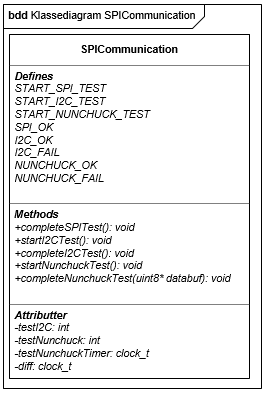
\includegraphics[]{DesignOgImplementering/images/SPICommunication}
	\caption{Klassediagram over klassen SPICommunication}
	\label{figure:KlassediagramSPICommunication}
\end{figure}
\subsubsection{Klassebeskrivelser}
I dette afsnit vil klassens metoder og defines blive beskrevet.
\newline

\noindent\textbf{void completeSPITest()} \newline
Denne metode gemmer \textit{SPI\_OK} i PSoC'ens SPI-transfer buffer. \newline

\noindent\textbf{void completeI2CTest()} \newline
Denne metode gennemfører I2C-Testen. Dette gøres ved at der sendes en besked til alle enheder på I2C-nettet, og hvis der ikke registreres nogen fejl på denne besked, bliver \textit{I2C\_OK} gemt i PSoC'ens SPI-transfer buffer. Registreres der en fejl, bliver \textit{I2C\_FAIL} gemt i SPI-transfer buffer. \newline

\noindent\textbf{void completeNunchuckTest(uint8* databuf)} \newline
Denne metode gennemfører Nunchuck-testen. Dette gøres ved at der startes en timer på 6 sekunder. Hvis der sker et tryk på 'Z'-knappen på nunchucken indenfor disse 6 sekunder, vil \textit{NUNCHUCK\_OK} blive gemt i SPI-transfer bufferen. Hvis der ikke registreres nogen tryk inden for de 6 sekunder, er det \textit{NUNCHUCK\_FAIL} der gemmes.\newline

I klassediagrammet er der beskrevet en række "Defines". Disse defines bruges i klassen som unikke ID'er der indikerer om en test er gennemført OK eller om den er fejlet.

\section{PSoC Software}
PSoC0 og PSoC1 gør begge brug af den tidligere beskrevne software. De følgende klassediagrammer figur \ref{figure:klassediagramPSoC0} og \ref{figure:klassediagramPSoC1} giver et overblik over hvilke klasser der bliver gjort brug af på de forskellige PSoCs

\begin{figure}[H]
	\centering
	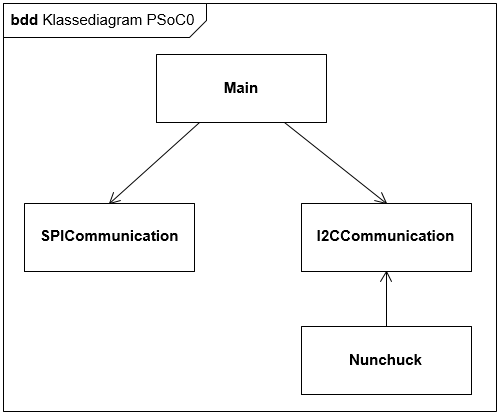
\includegraphics[width=.7\textwidth]{DesignOgImplementering/images/PSoC0KlassediagramOversigt}
	\caption{Klassediagram oversigt for PSoC0}
	\label{figure:klassediagramPSoC0}
\end{figure}

\begin{figure}[H]
	\centering
	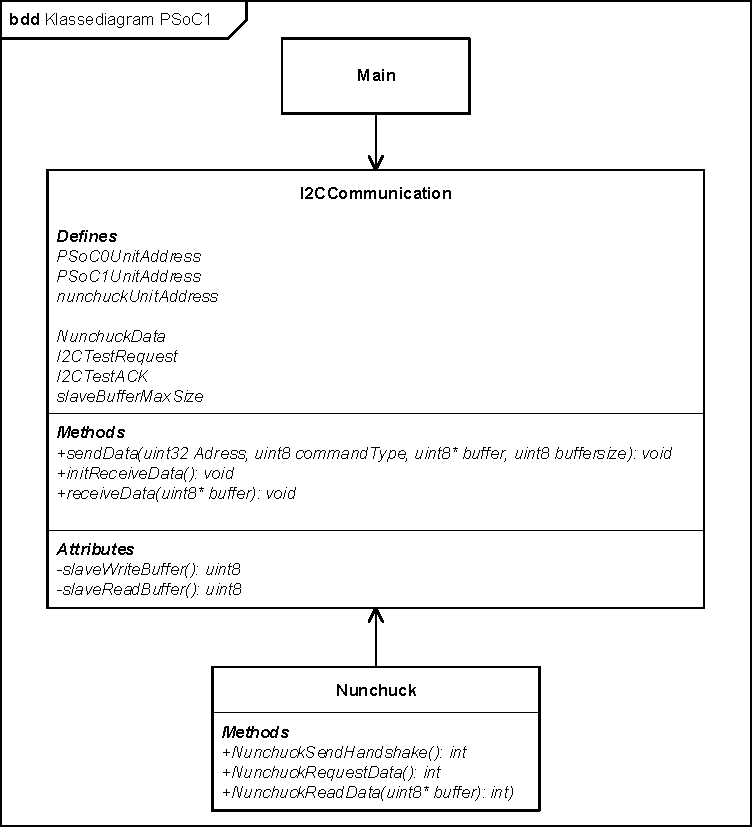
\includegraphics[width=.7\textwidth]{DesignOgImplementering/images/PSoC1KlassediagramOversigt}
	\caption{Klassediagram oversigt for PSoC1}
	\label{figure:klassediagramPSoC1}
\end{figure}

\subsection{SPI - Devkit8000}
Candydriveren sørger for SPI-kommunikationen fra Devkit8000 til PSoC0. Driveren er skrevet i c, hvilket er typisk for drivere til linuxplatforme.\\
SPI-kommunikationen er implementeret med SPI bus nummer 1, SPI chip-select 0 og en hastighed på 1 MHz (et godt stykke under max på 20 MHz for en sikkerhedsskyld). Desuden starter clocken højt og data ændres på falling edge og aflæses på rising edge. Dermed bliver SPI Clock Mode 3. Derudover sendes der 8 bit pr transmission, hvilket passer med SPI-protokollen for projektet.\\
For at kunne anvende driveren, når SPI er tilsluttet, er der oprettet et hotplugmodul, som fortæller kernen, at der er et SPI device, som matcher driveren. Det kan SPI-forbindelsen ikke selv gøre, som usb fx kan. Selve driveren er i candygun.c opbygget som en char driver. For at holde forskellige funktionaliteter adskilt er alle funktioner, der har med SPI at gøre, implementeret i filen candygun-spi-c. Så når der fx skal requestes en SPI ressource i init-funktionen i candygun.c, så anvender driveren en funktion fra candygun-spi.c til det. I probe-funktionen sættes bits\textunderscore per\textunderscore word til 8, da vi sender otte bit som nævnt tidligere. I exit-funktionen anvender candygun.c igen en funktion fra candygun-spi.c - denne gang til at frigive SPI ressourcen. I write-metoden gives der data med fra brugeren. I dette tilfælde udgøres brugeren af Interface driveren og dataet er en 8 bit kommando fra SPI-protokollen. Dog er dataet fra brugeren i første omgang læst ind som en charstreng. I write-metoden bliver det så lavet om til en int.  For at overføre dataet på en sikker måde anvendes funktionen copy\textunderscore from\textunderscore user() til at overføre data fra brugeren. Write-funktionen fra candygun.c anvender derefter en write-funktion fra candygun-spi.c, hvor den sender brugerinputtet med. I den spi-relaterede write-funktion bliver bruger inputtet lagt i transfer bufferen og der NULL bliver lagt i receive bufferen, og med spi\textunderscore sync-funktionen bliver det sendt.\\ 
Ofte ville der en spi read-funktion først indeholde en write-del, som fortalte SPI-slaven, hvad der skulle læses over i bufferen. Det ville typisk efterfølges af et delay og så en read-del. Men i dette projekt skal der ofte afventes et brugerinput, som ikke kan styres af et fast delay, og der skal generelt sendes en aktiv kommando før der læses. Derfor er det besluttet at read-funktionen kun indeholder en read-del i transmissionen. Dermed skal write-funktionen altid aktivt anvendes inden der læses, da PSoC0 ellers ikke ved, hvad der skal gøres/lægges i bufferen.\\
Når funktionen har modtaget resultatet fra transmissionen returneres det til brugeren med funktionen copy\textunderscore to\textunderscore user(), som igen sørger for at overførslen af data foregår på en sikker måde.   


\subsection{Interface Driver}
Interface driveren fungerer som bindeled mellem brugergrænsefladen og candydriveren på Devkit8000. Den indeholder tre funktioner. Funktionerne anvendes i use case 2 til at teste kommunikationsforbindelserne i resten af systemet. Interface driveren er designet og implementeret i C++ og gør brug af klasserelationen arv. Et klassediagram for interface driveren se på figur  \ref{fig:idriveruc2}.\\

\begin{figure}[H]
	\centering
	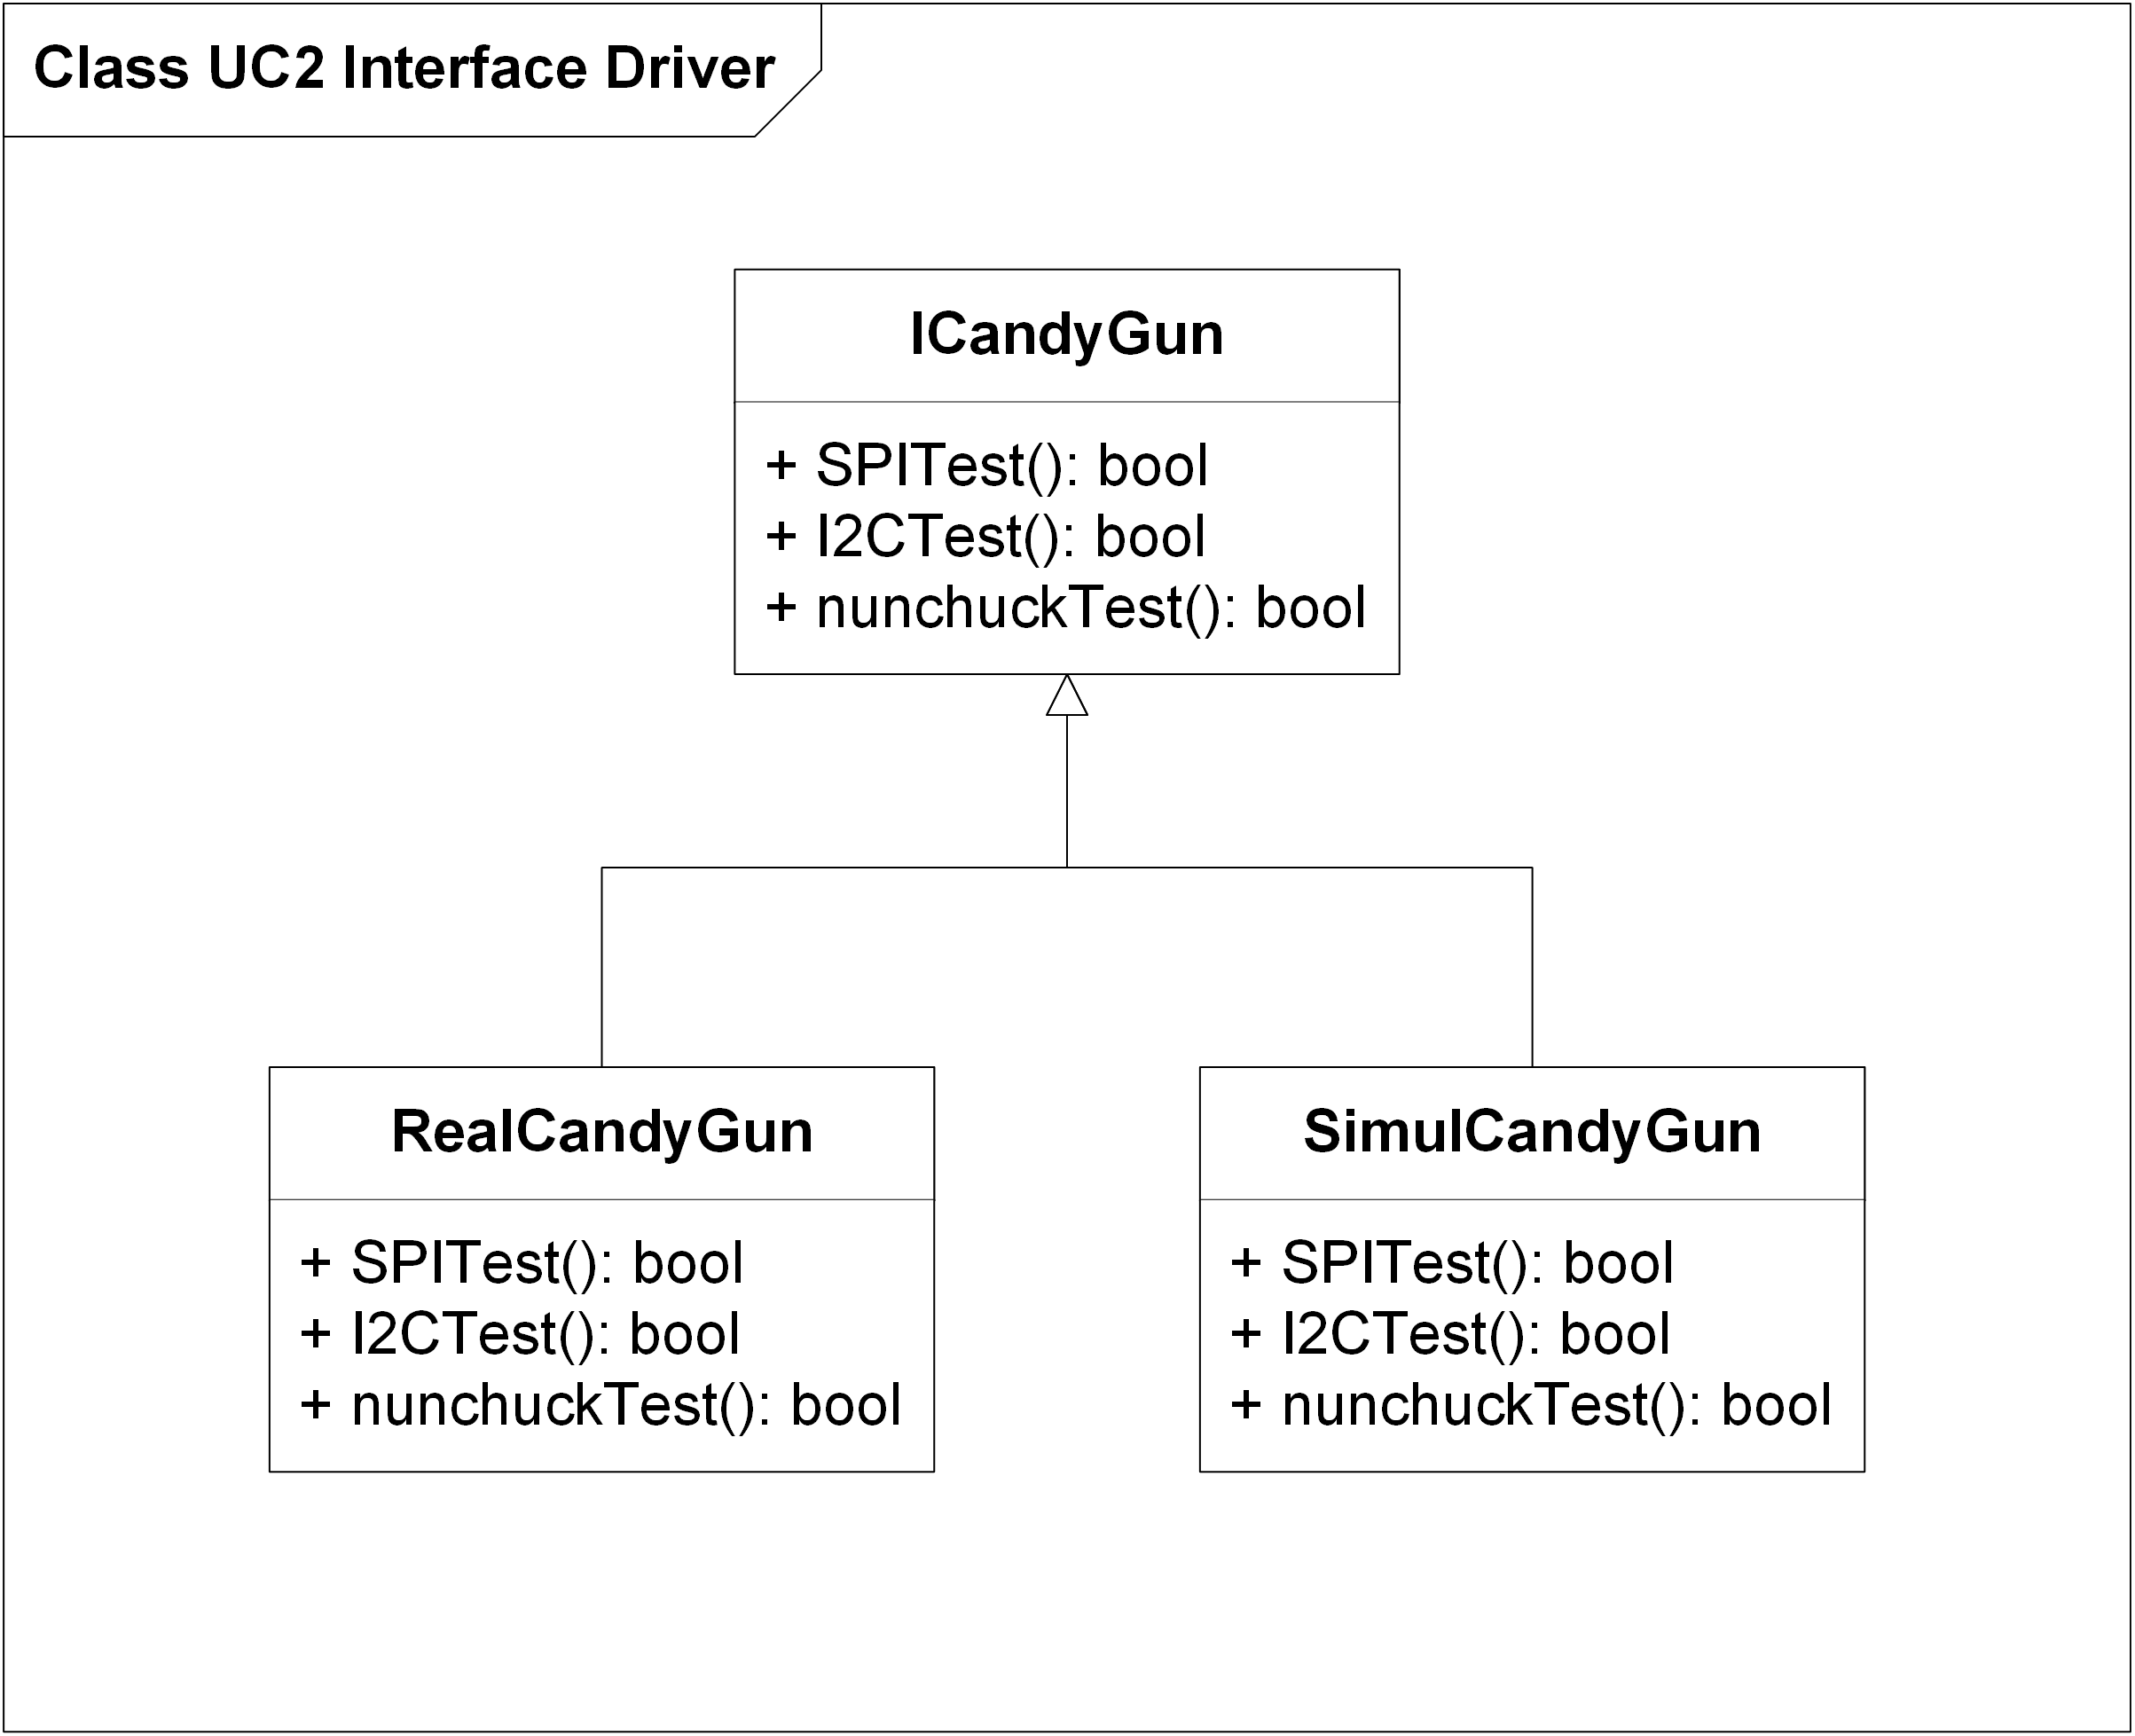
\includegraphics[width=\textwidth]{Afsnit/DesignOgImplementering/images/IdriverKlasseDiagram}
	\caption{Interface driver for UC2}
	\label{fig:idriveruc2}
\end{figure}

Basisklassen er ICandyGun. Det er en abstrakt klasse, da den udelukkende indeholder virtuelle metoder. Derudover er der to afledte klasser; SimulCandyGun og RealCandyGun. SimulCandyGun implementerer metoderne til at simulere respons fra Candydriveren. Dermed kan brugergrænsefladen testes uafhængigt af de resterende dele af systemet. Simuleringen er implementeret med \textit{srand()}-funktionen fra \textit{cstdlib}-biblioteket, som returnerer et tilfældigt tal, som her bliver mellem 0 og 1. I RealCandyGun-klassen er metoderne implementeret efter den reelle SPI-protokol og med de nødvendige funktioner til at skrive til et kernemodul. Fx open(), close(), read () og write(). Da interface driveren er implementeret med arv, skal der ikke foretages betydelige ændringer i brugergrænsefladen, når der skiftes mellem simuleringsklassen og den rigtige version. Dermed opnås lav kobling. \\
De tre funktioner som Interface driveren indeholder i forbindelse med use case 2 (test use casen) er: SPITest(), I2CTest(), NunchuckTest(). Hver af de tre funktioner anvendes til at starte en test af de forskellige kommunikationsforbindelser: SPI, I2C og brugerinputet fra nunchucken. Alle funktionerne returnerer en bool, som enten er true eller false, alt efter om testen var succesful eller ej. Når der skal startes en test, åbner den pågældende funktion filen \textit{dev/candygun} og skriver SPI-kommandoen for \textit{start test} til filen. Derefter venter funktionen ét sekund og læser så svaret fra filen. Da der i nunchucktesten ventes på et brugerinput, og brugeren skal have lidt tid til at trykke på nunchuck-knappen, er der oprettet en while-løkke, som tjekker flere gange om testen returnerer true. Hvis testen ikke returnerer true ved første check, venter funktionen atter et sekund og tjekker igen. Det gør den op til 15 gange og melder derefter om fejl, hvis ikke den returnerer true inden.\\
Brugergrænsefladen anvender interface driveren ved at inkludere headerfilerne og oprette en ICandyGun pointer, der peger på en instans af én af de to afledte klasser. Ved at pakke kommunikationen  til kernemodulet for candydriveren væk i funktioner kan brugergrænsefladen anvende funktionerne uden at kende til SPI-protokollen. Det sikrer igen lav kobling, og i tilfælde hvor det kunne ønskes, at SPI-kommunikationen kan erstattes af en anden kommunikationsform, kan det gøres uden, at der skal foretages ændringer i brugergrænsefladen.\\
 
\subsection{Brugergrænseflade}
\begin{figure}[H]
	\centering
	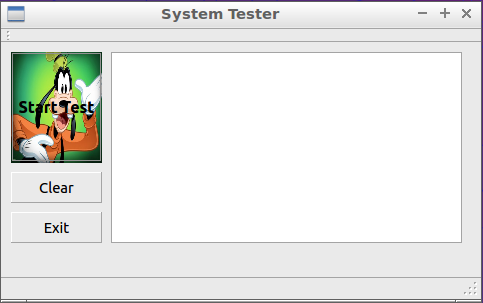
\includegraphics[width=\textwidth]{Afsnit/DesignOgImplementering/images/GUIPic}
	\caption{Brugergrænseflade for usecase 2}
	\label{fig:GUIPic}
\end{figure}

Brugergrænsefladen er lavet med det indbyggede design framework i QT Creator 5.
QT frameworket opretter "hovedvinduet" i brugergrænsefladen som en klasse. Knapperne tilføjes som private slots i klassen
hvilket gør dem i stand til interagere i brugergrænsefladen. Når en knap er assignet til et slot i klassen, og der trykkes på den pågældende knap, bliver det assignede signal broadcastet
og slot-funktionen bliver kørt. Alle tre knapper i brugergrænsefladen er assignet signal-typen "clicked()". Signalet broadcastets når knappen trykkes.

\begin{figure}[H]
	\centering
	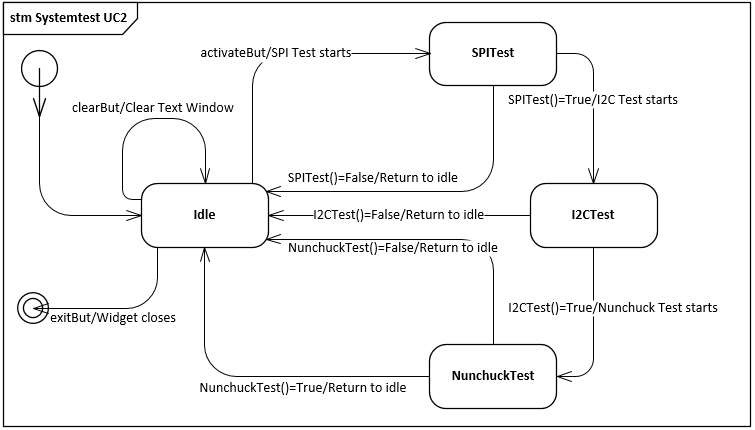
\includegraphics[width=\textwidth]{Afsnit/DesignOgImplementering/images/StateMachineUC2}
	\caption{State machine for brugergrænsefladen for usecase 2}
	\label{fig:StateMachineUC2}
\end{figure}

Brugergrænsefladen for UC2 er en simpel test-konsol. Den består af 3 knapper og et tekstvindue. Brugergrænsefladen interfacer med SPI-protokollen, gennem vores interface driver. Den første knap, Start test, initierer UC2. Efterhånden som testen løbes igennem kaldes test funktionerne, og ved hjælp af if-conditions, bliver der tjekket på retur-værdierne fra interface-funktionerne. Hvis retur-værdien er true, skrives der en "--test successful" besked i tekstvinduet. og widgeten kører videre. Hvis retur-værdien er false, skrives der en "--test unsuccessful" i tekstvinduet og widgeten returnerer til idle tilstand. Når alle test er successful, skrives "System test successful, system is ready for use" til tekstvinduet, og widgeten returnerer til idle tilstand. Den anden knap, Clear, clearer tekstvinduet til blank tilstand. Den tredje knap, Exit, lukker widgeten.